For the first analysis, we considered the original dataset located at \url{http://www.lpthe.jussieu.fr/~erbin/files/data/}: the file was last downloaded on February, 24th 2020 and never directly modified. Before moving to the application of machine learning algorithms and neural networks, we first visualised and analysed the available data in order to extract usable features and gain some insights to be used in the following analysis.

In what follows we use \textit{Scikit-learn} (v.\ 0.22.1), \textit{XGBoost} (v.\ 0.90) and \textit{Keras} (v.\ 2.3.1, with \textit{Tensorflow} v.\ 2.0.0 backend) as reference libraries in a \textit{Conda} installation on \textit{Arch Linux}. Hardware specifications are as follow:
\begin{itemize}
    \item CPU: Intel Core i7-7700HQ @ 2.80 GHz,
    \item GPU: NVIDIA GeForce 940 MX (2 GB RAM),
    \item RAM: 16 GB.
\end{itemize}

\subsection{Data Visualisation}

    After loading the dataset, as a first approach, we considered the distribution in the number of occurrences of $h_{11}$ and $h_{21}$. We considered only manifolds which cannot be represented as products of spaces and we removed some outliers: we considered therefore only entries whose column \texttt{isprod} is identically $0$ and we kept the Hodge numbers in the range $h_{11} \in \left[ 1, 16 \right]$ and $h_{21} \in \left[1, 86 \right]$. We show in Figure~\ref{fig:distribution_occurrences} the distribution of occurrences thus derived. We will then consider the dataset without outliers and product spaces in the following analysis.
    
    \begin{figure}[!t]
        \centering
        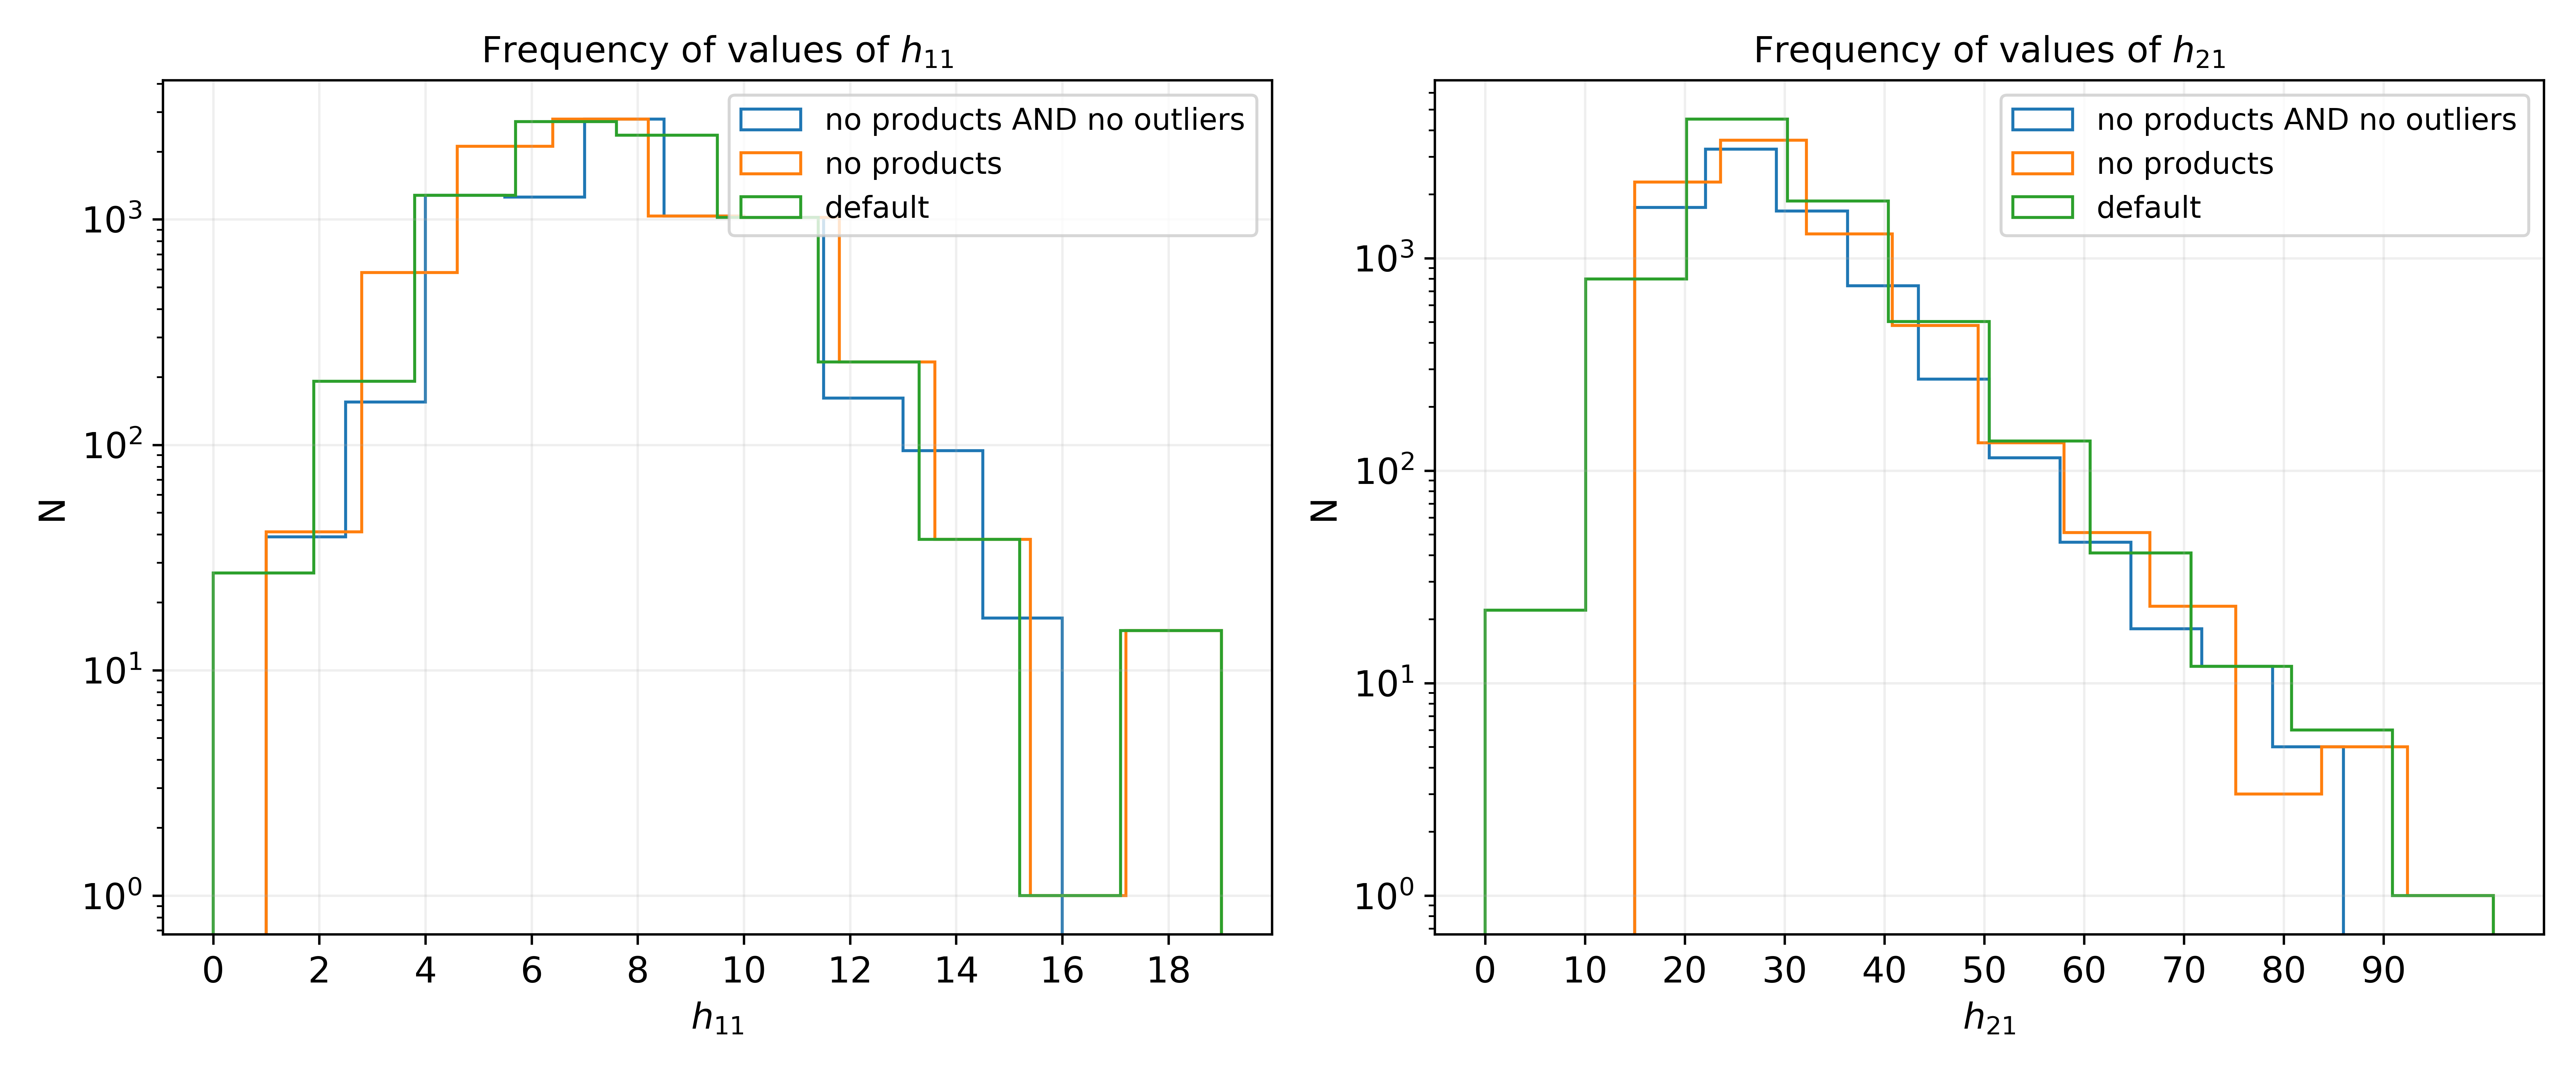
\includegraphics[width=\textwidth]{tex/img/h11_h21_occurrencies.png}
        \caption{Distribution in the number of occurrences of $h_{11}$ and $h_{21}$. The original untouched dataset, the dataset without product spaces and the dataset without outliers are shown in different colours.}
        \label{fig:distribution_occurrences}
    \end{figure}
    
    As a reference, we also plot the distribution of $h_{11}$ and $h_{21}$ with respect to some of the features. Specifically we used \texttt{num\_cp}, \texttt{num\_eqs}, \texttt{norm\_matrix} and \texttt{rank\_matrix} as a reference: relations shown Figure~\ref{fig:scatter_plot_distributions} are not always linear but the distributions of $h_{11}$ and $h_{21}$ show however a tendency to correlation more than sparsity.
    
    \begin{figure}[!t]
        \centering
        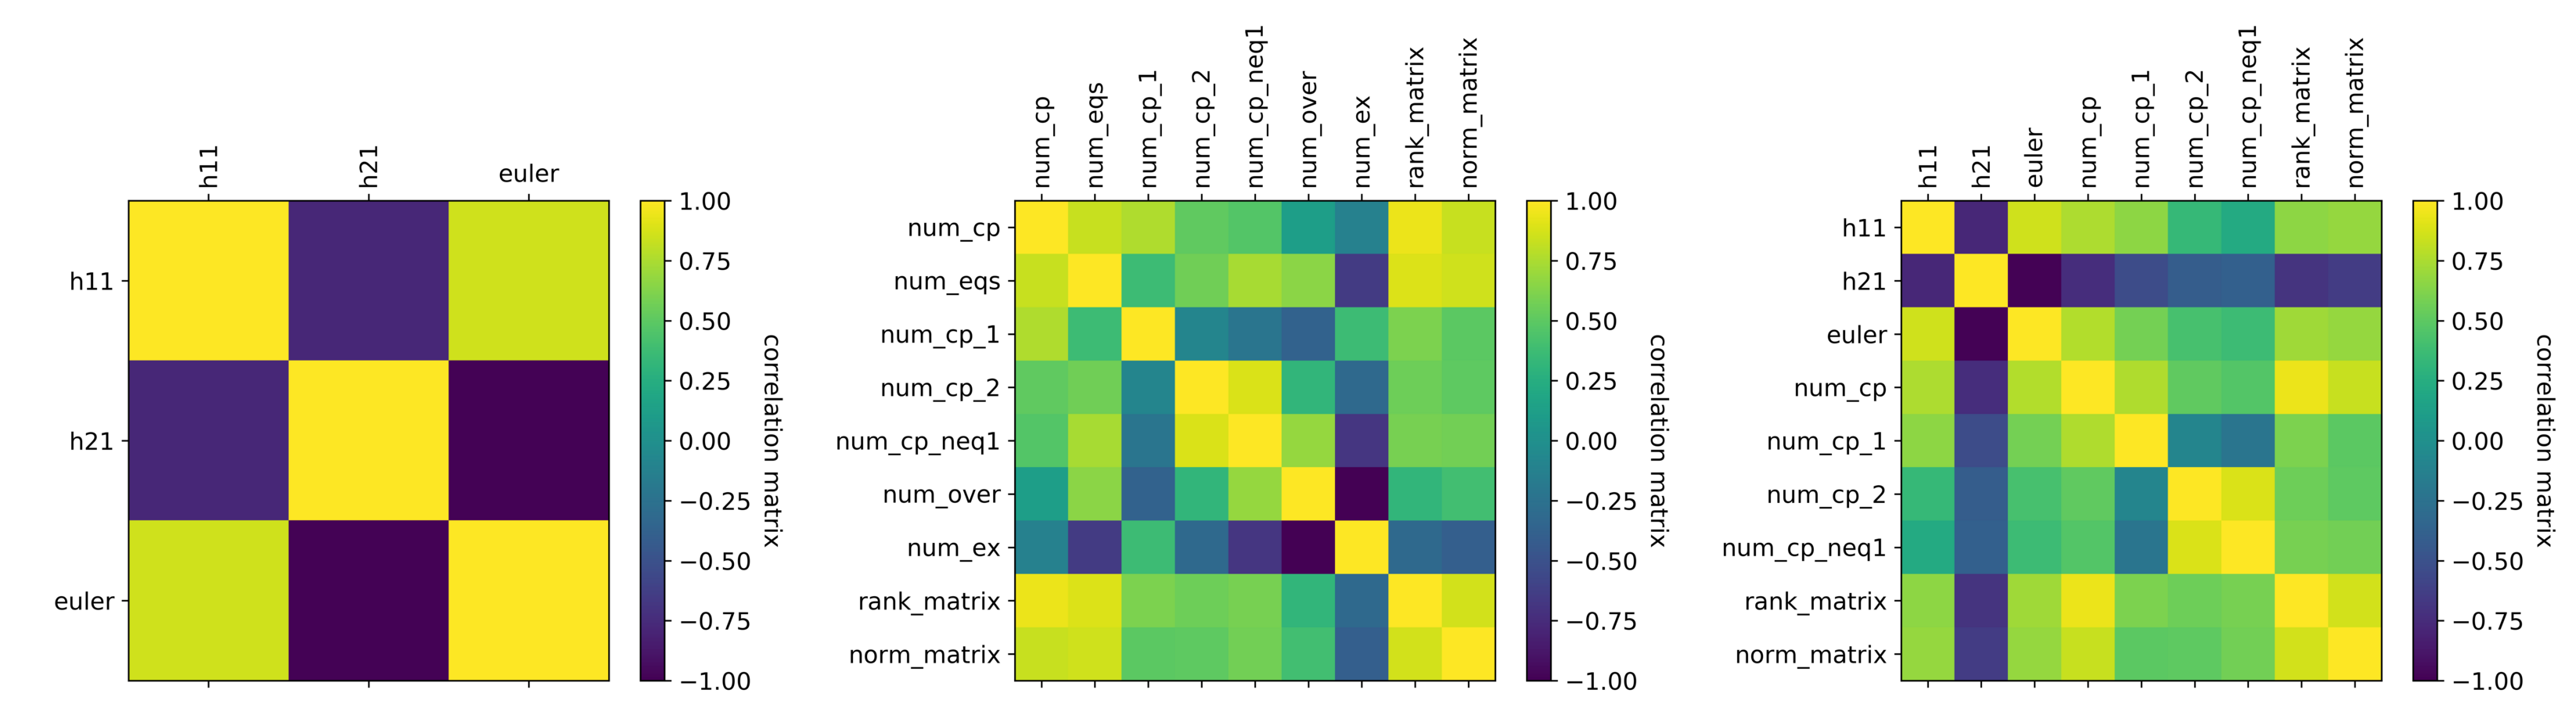
\includegraphics[width=\textwidth]{tex/img/correlation_matrix.png}
        \caption{Correlation matrix of the (scalar) features.}
        \label{fig:correlation_matrix}
    \end{figure}
    
    This can also be inferred from the correlation matrix in Figure~\ref{fig:correlation_matrix} which shows the relations between the labels \texttt{h11}, \texttt{h21} and \texttt{euler} (the latter will not be considered in the analysis) and with respect to other scalar features.
    
    \begin{figure}[p]
        \centering
        \includegraphics[height=0.9\textheight,
                         trim={0 0 6in 0},
                         clip
                        ]{tex/img/h11_h21_distributions.png}
        \caption{Distribution of $h_{11}$ and $h_{21}$ with respect to a restricted number of available features.}
        \label{fig:scatter_plot_distributions}
    \end{figure}
    
\subsection{Clustering and PCA}

    To improve the predictive abilities of the algorithms, we employ a clustering analysis (unsupervised) on the components of the configuration matrix in the hope to find possible associations amongst the entries of the dataset. Since we are not interested in predictions, we use the entire dataset and consider the assigned labels as a new feature for the dataset. In particular we considered K-Means clustering using the \texttt{KMeans} algorithm (\texttt{random\_state} = 42). We ran the algorithm several times in a range of clusters between 2 and 19 and added the labels to the dataset to be later analysed.
    
    \begin{figure}[!t]
        \centering
        \includegraphics[width=\textwidth]{tex/img/h11_h21_pca_distribution.png}
        \caption{Principal Components Analysis with two components on the entire dataset.}
        \label{fig:pca_analysis}
    \end{figure}
    
    We then moved to the Principal Components Analysis (unsupervised) of the components of the configuration matrix using the algorithm \texttt{PCA} (\texttt{random\_state} = 42). We first considered the case of only 2 principal components to be used in plots but not in the real analysis. We show in Figure~\ref{fig:pca_analysis} the distribution of $h_{11}$ and $h_{21}$ with respect to such components. For the analysis we focused on keeping the 99\% of the total variance which, from a $12 \times 15$ (180 entries) matrix, led to a vector of 81 components.
    
\subsection{Feature Importances}

    Using the engineered features (including clustering and PCA), we then train a \texttt{RandomForestRegressor}, using the \textit{Scikit-learn} implementation, on the entire dataset (we are still not interested in making predictions) to measure the variable ranking for the different features. The algorithms does not need to be fine tuned at this level of the analysis. We therefore considered the following hyperparameter space\footnote{Here as in the following, hyperparameter which are not explicitely specified are to be considered at their defaults.}:
    \begin{itemize}
        \item \texttt{criterion}: \textit{mse},
        \item \texttt{n\_estimators}: 48,
        \item \texttt{random\_state}: 42.
    \end{itemize}
    Even though it is not relevant for the analysis for many reasons (one above all, it was not computed on a separate training set from which to validate the results before making prediction), the accuracy for $h_{11}$ resulted to be $90.74\%$ and $59.00\%$ for $h_{21}$.
    
    \begin{figure}[!t]
        \centering
        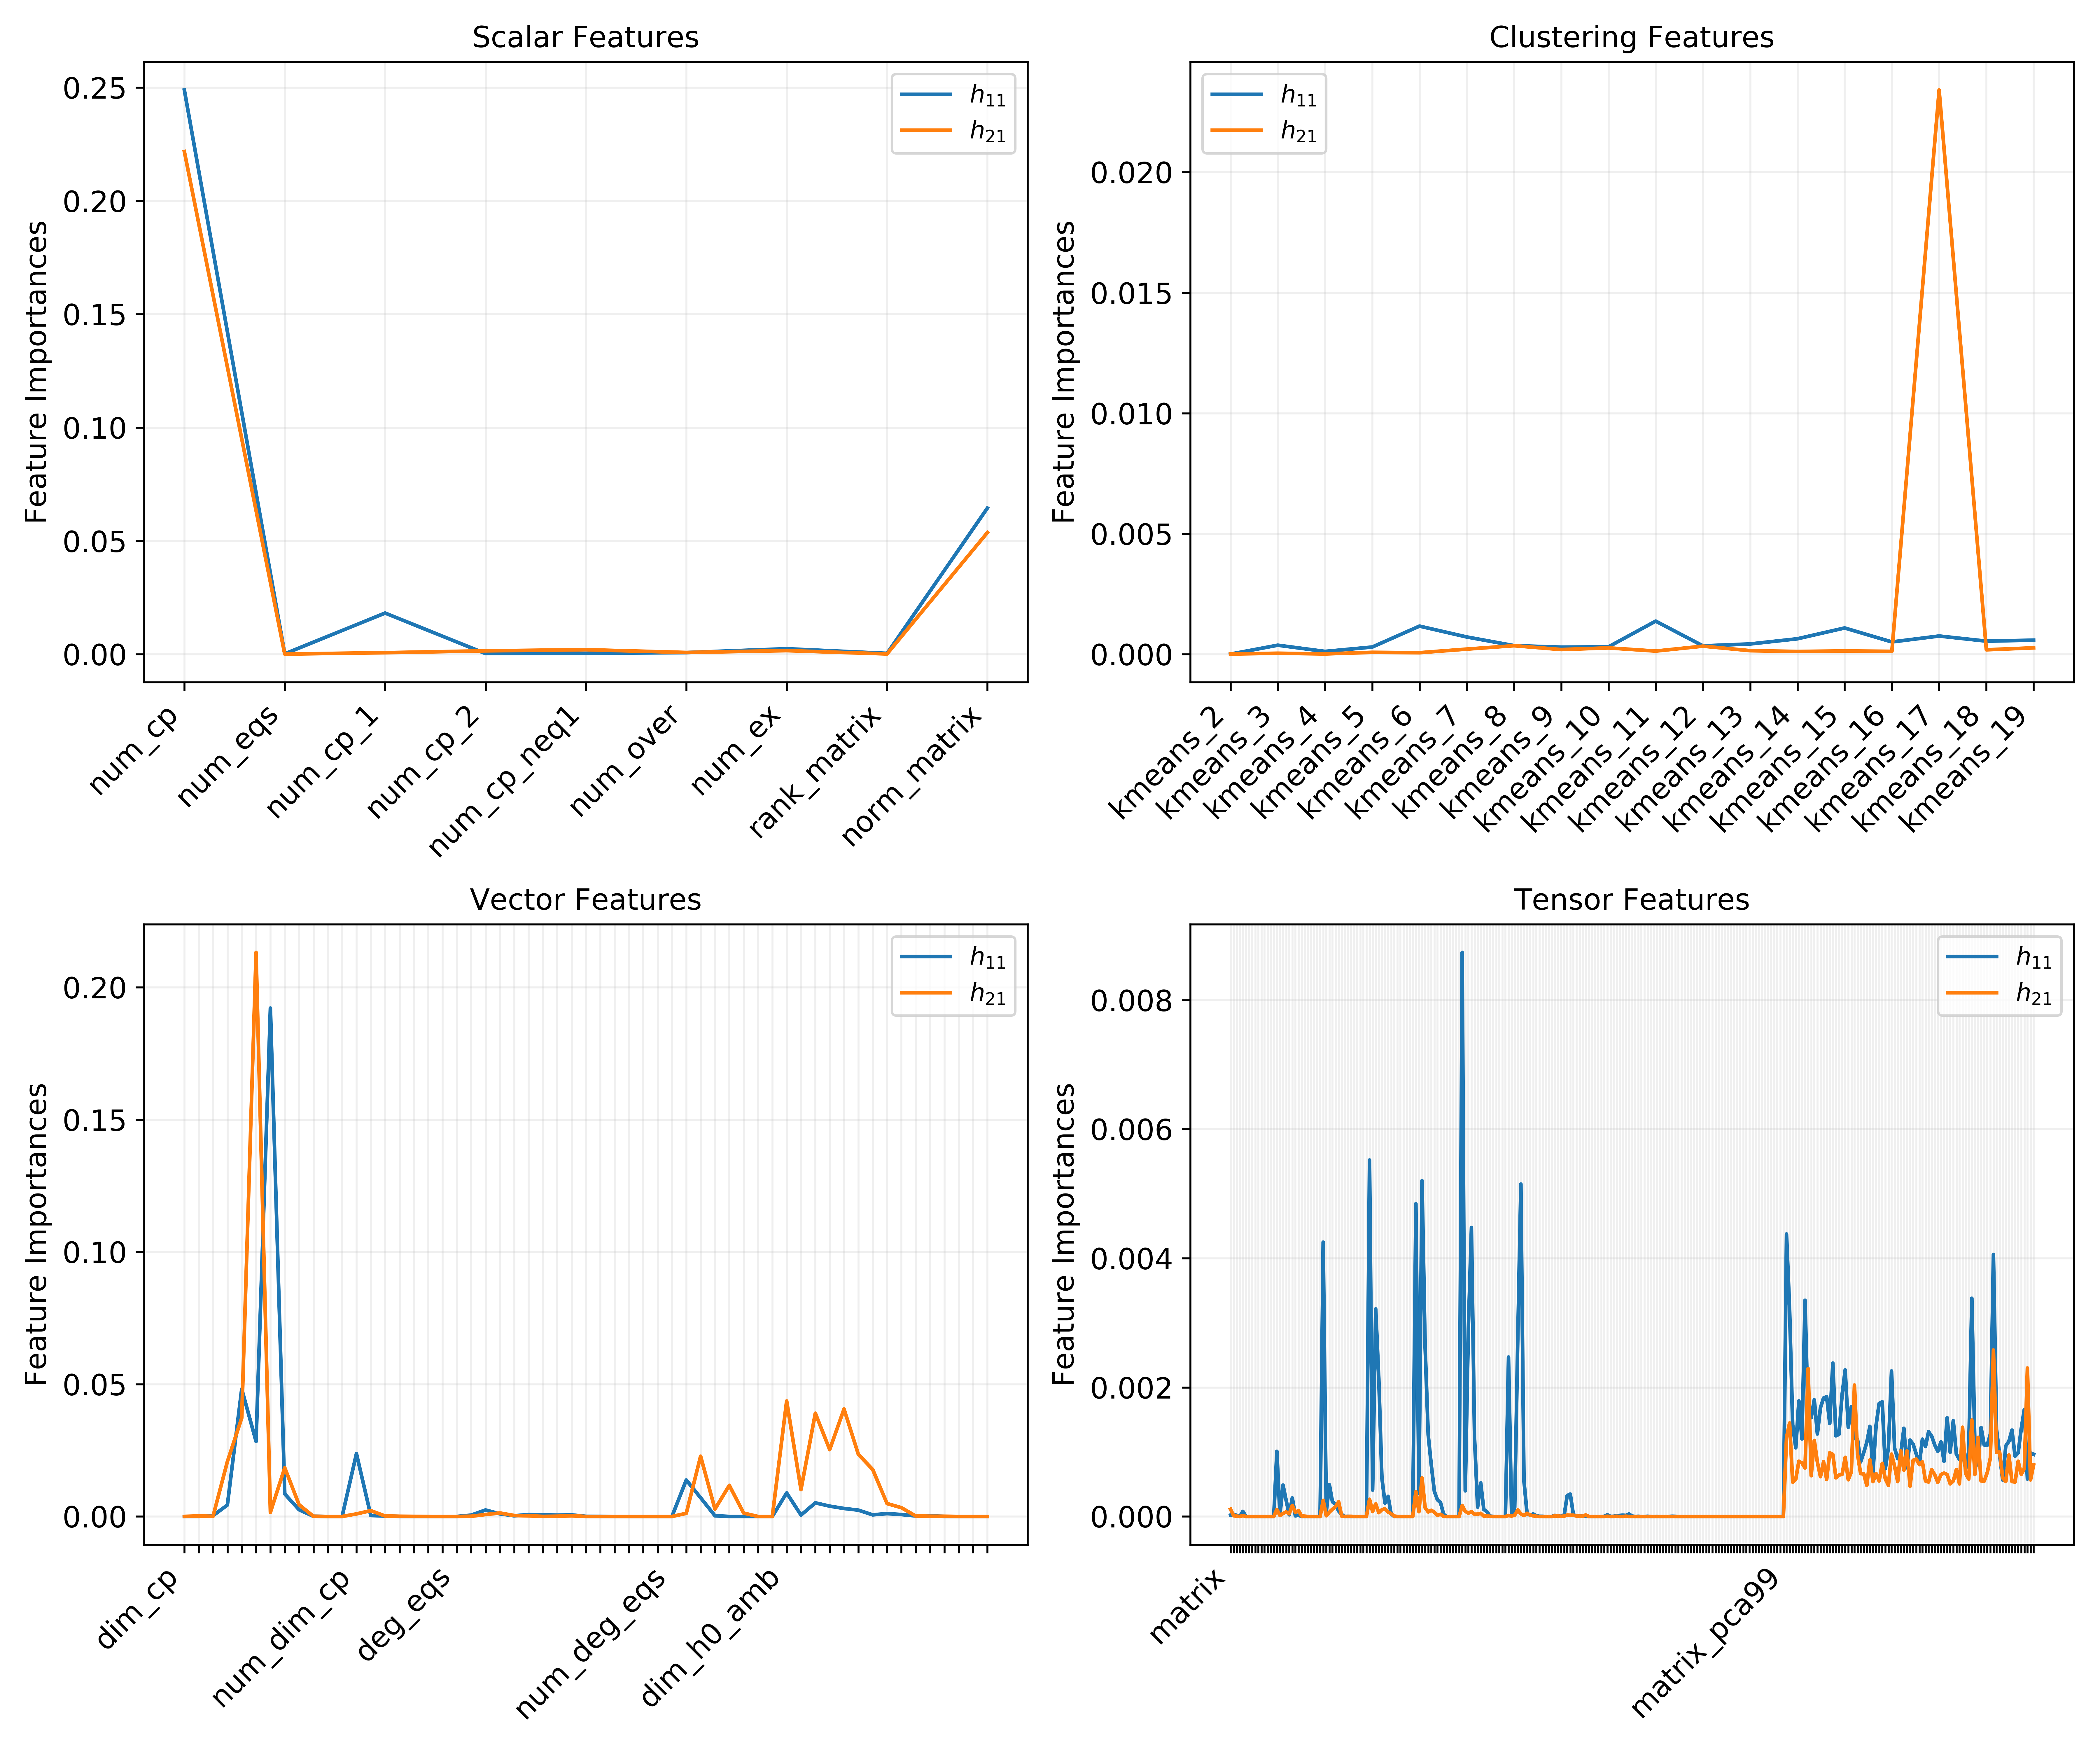
\includegraphics[width=0.75\textwidth,
                         trim={6in 5in 0 0},
                         clip
                        ]{tex/img/feature_importances.png}
        \caption{Clustering ranking.}
        \label{fig:clustering_importances}
    \end{figure}
    
    In Figure~\ref{fig:clustering_importances} we show the ranking of the clustering algorithm which shows that \texttt{KMeans} does not play a role in the prediction of $h_{11}$ while it is only marginally relevant for $h_{21}$. The number of clusters needed is however unrelated to any other feature and varies a lot in relation to the random seed initially set (42 in the case reported here).
    
    \begin{figure}[!t]
        \centering
        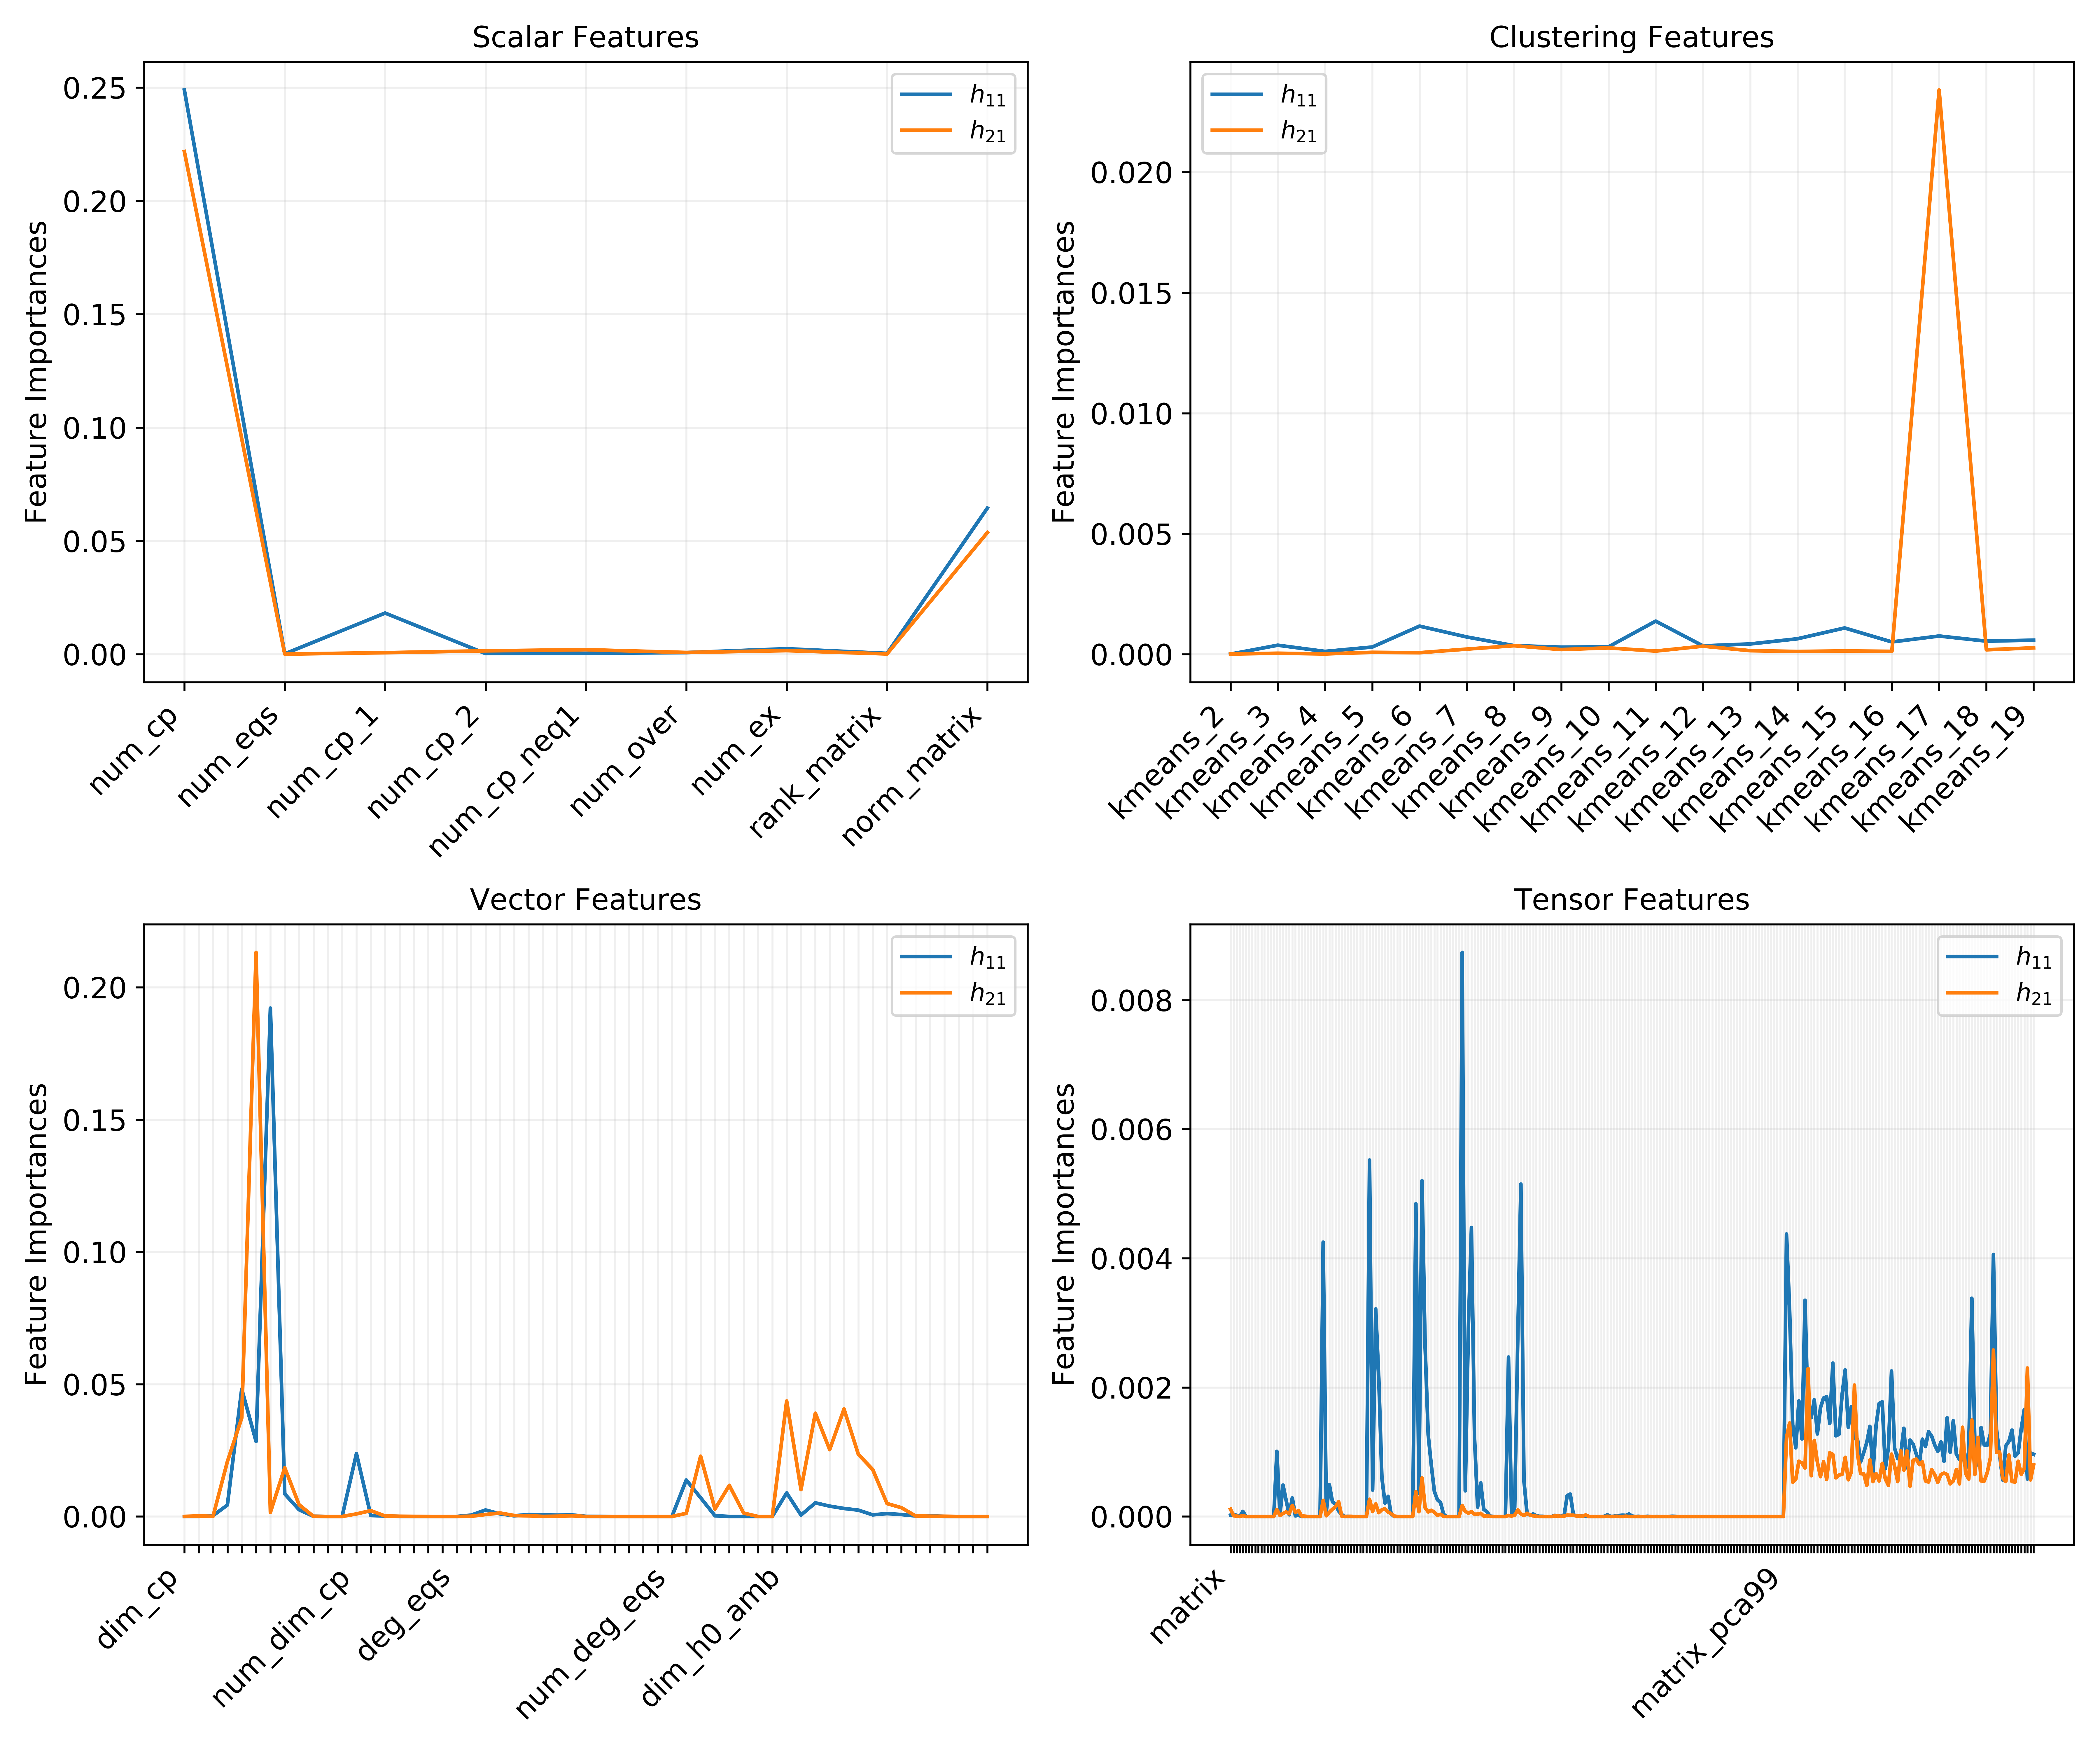
\includegraphics[width=0.75\textwidth,
                         trim={0 5in 6in 0},
                         clip
                        ]{tex/img/feature_importances.png}
        \caption{Scalar ranking.}
        \label{fig:scalar_importances}
    \end{figure}
    
    \begin{figure}[!t]
        \centering
        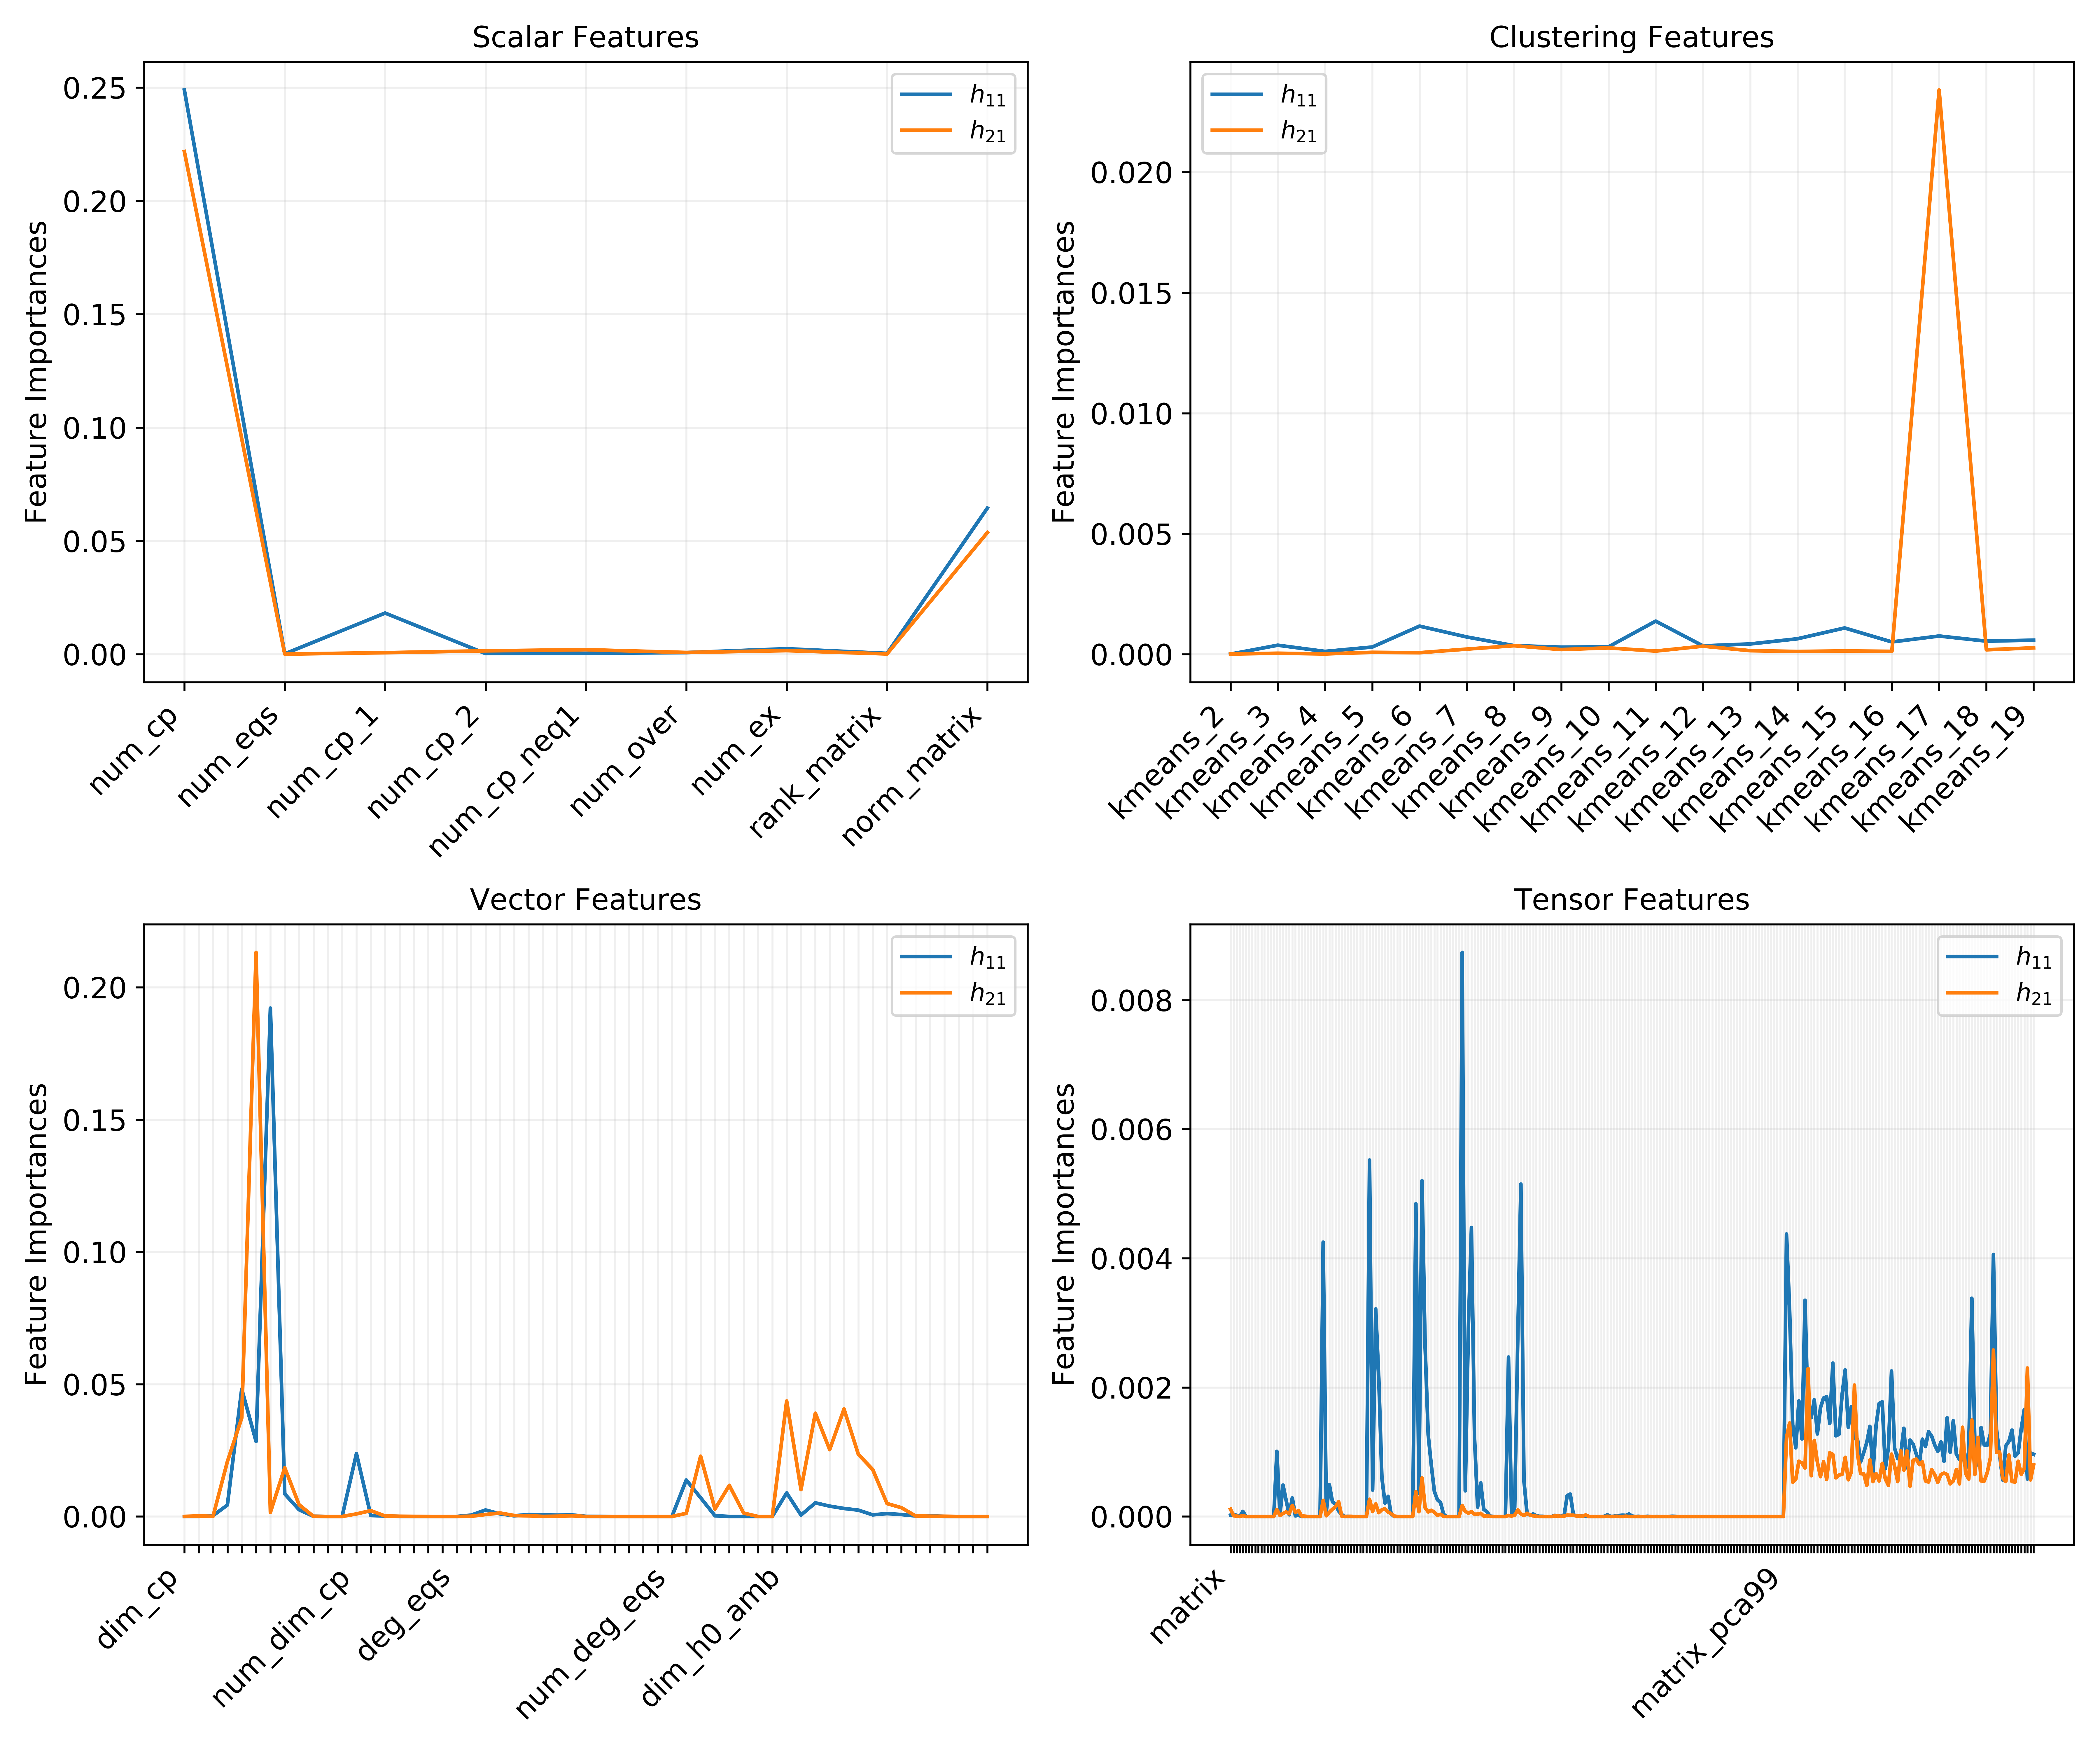
\includegraphics[width=\textwidth,
                         trim={0 0 0 5in},
                         clip
                        ]{tex/img/feature_importances.png}
        \caption{Vector and tensor ranking.}
        \label{fig:vector_tensor_importances}
    \end{figure}
    
    \begin{figure}[!t]
        \centering
        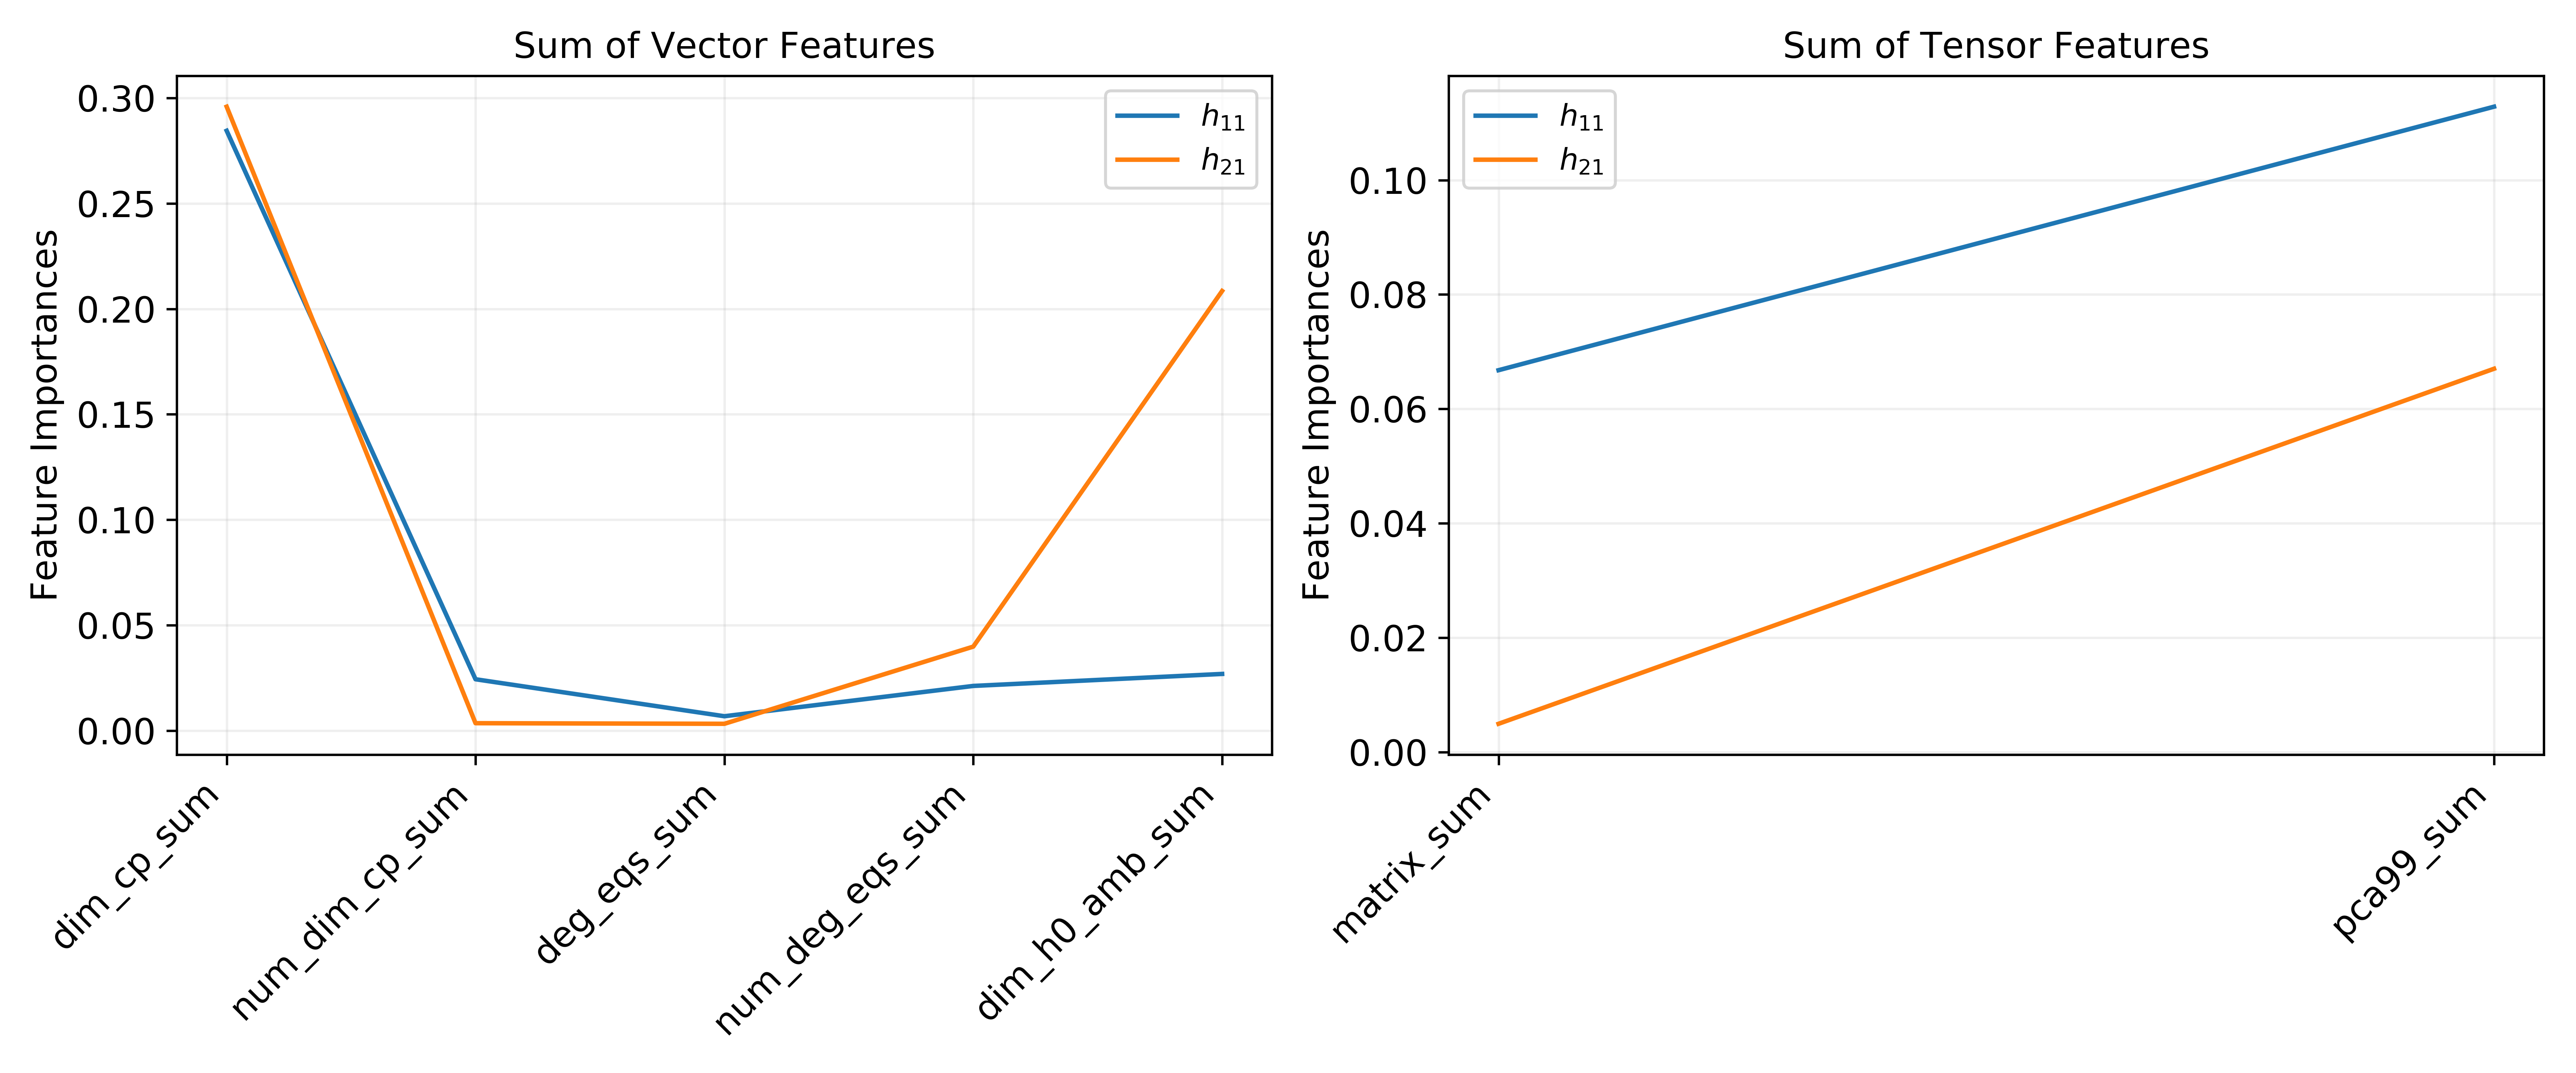
\includegraphics[width=\textwidth]{tex/img/feature_importances_vector_tensor_sum.png}
        \caption{Sum of vector and tensor ranking.}
        \label{fig:vector_tensor_sum_importances}
    \end{figure}
    
    In Figure~\ref{fig:scalar_importances} we show the importance related to the other scalar features, thus showing that only a few of them will actually play a relevant role in the determination of the labels. The same also applies to the vector and tensor features (shown in Figure\ref{fig:vector_tensor_importances} by components): while it may be simpler to show the sum of the importance of the components (as in Figure~\ref{fig:vector_tensor_sum_importances}), it is already clear that the \texttt{PCA} is more relevant than the plain matrix. We then show in Figure~\ref{fig:summary_importances} a summary of the variable ranking.
    
    \begin{figure}[!t]
        \centering
        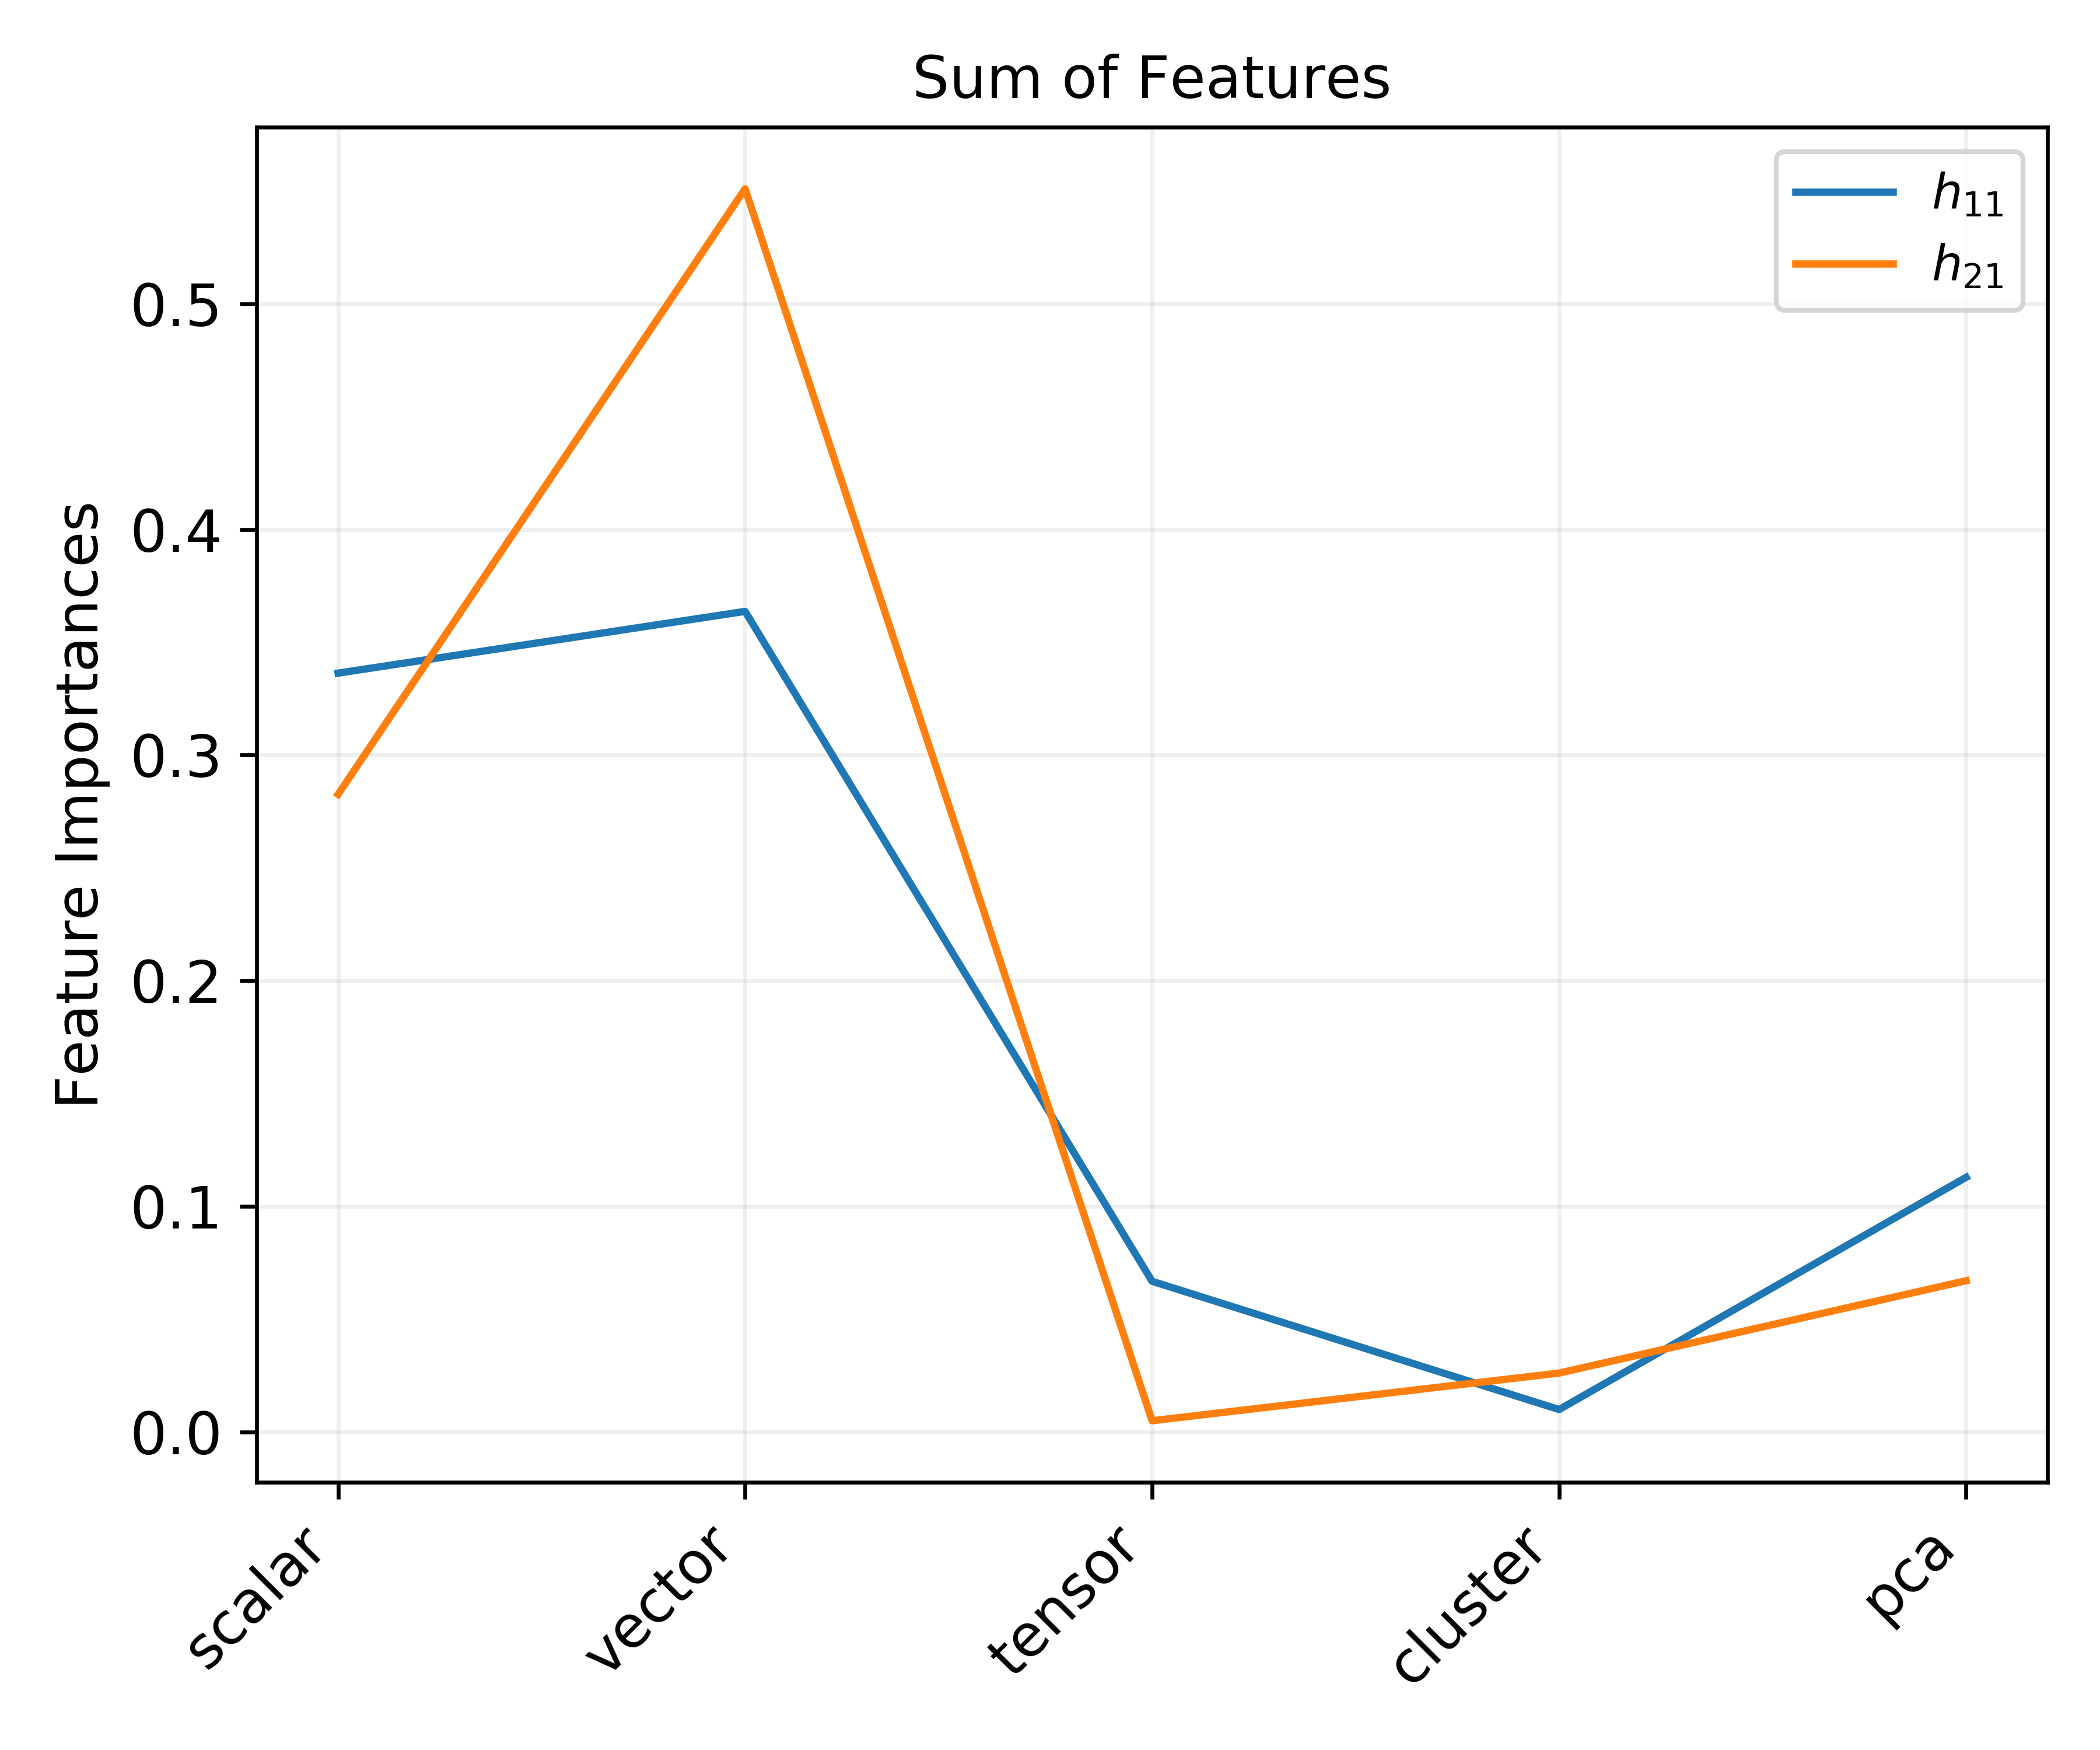
\includegraphics[width=0.75\textwidth]{tex/img/feature_importances_sum.png}
        \caption{Summary of the variable ranking}
        \label{fig:summary_importances}
    \end{figure}
    
\subsection{Feature Selection}

    Using previous results, we then select only the relevant features for the following analysis. In particular we select \texttt{num\_cp}, \texttt{dim\_cp} and the \texttt{PCA} of the configuration matrix for the predictions of $h_{11}$ and \texttt{num\_cp}, \texttt{dim\_cp}, \texttt{dim\_h0\_amb} and the \texttt{PCA} of the configuration matrix for the predictions of $h_{21}$. However we also keep a separate copy of the configuration matrix, \texttt{num\_cp} only and \texttt{dim\_cp} only for comparison during the analysis.